%! TEX program = xelatex
%       File: VTthesis_template.tex
%     Created: Thu Mar 24 11:00 AM 2016 EDT
%     Last Change: August 15, 2024
%     Author: Alan M. Lattimer, VT
%	  With modifications by Carrie Cross, Robert Browder, and LianTze Lim. 
%
% This template is designed to operate with XeLaTeX.
%
% All elements in the Title, Abstract, and Keywords MUST be formatted as text and NOT as math.
%
%Further instructions for using this template are embedded in the document. Additionally, there are comments at the end of the file that give suggestions on writing your thesis.  
%
%In addition to the standard formatting options, the following options are defined for the VTthesis class: proposal, prelim, doublespace, draft. 

\documentclass[doublespace,nopageskip]{VTthesis} % nopageskip - Removes arbitrary blank pages.

% Using the following header instead will create a draft copy of your thesis
%\documentclass[doublespace,draft]{VTthesis}

% The lipsum package is just included to put dummy text in the document in order to demonstrate page headers and table of contents behavior. You should remove it once you begin writing your actual thesis or dissertation.
\usepackage{lipsum}
\usepackage{array}
\usepackage{graphicx}
\usepackage[export]{adjustbox}
\graphicspath{ {./images/} }

% Title of your thesis
\title{
Neuro-Symbolic Reinforcement Learning: A Reinforcement Learning Platform \& Neuro-Symbolic Agent}

% You should include 3-5 keywords, separated by commas
\keywords{Reinforcment Learning, Neuro-symbolic, Neuro-symbolic Concept Learner, Multi-task Reinforcement Learning, Robotics}

% Your name, including middle initial(s)
\author{Hunter W. Ellis}

% Change this to your program, e.g. Physics, Civil Engineering, etc.
\program{Computer Engineering} 

% Change this to your degree, e.g. Master of Science, Master of Art, etc.
\degree{Master of Science} 

% This should be your defense date:
\submitdate{March 23, 2016} 

% Committee members. Only have five readers and one chair available.
% Only use the ones you need and don't include the ones you don't need.
% You can also declare a Co-advisor. Per the VT ETD standards, 
% you should not include titles such as Dr. or Professor, but can list educational 
% qualifications after the name (i.e., John Doe, MFA or Jane Smith, PhD)
% Names should appear as they do in ESS/Banner/HokieSpa, including middle initials.
\principaladvisor{Thinh T. Doan, PhD}
\coadvisor{Michael S. Hsiao, PhD}
\firstreader{Ryan K. Williams, PhD}
%\secondreader{Kara M. Jones}
%\thirdreader{James Smith}
%\fourthreader{Fourth Committee Member}
%\fifthreader{Fifth Committee Member}

% The dedication and acknowledgement pages are optional. Comment them out to remove them.
\dedication{This is where you put your dedications.}
\acknowledge{This is where you put your acknowledgement.}
%\acknowledge{Thank you to Dr. Thinh Doan and Dr. Michael Hsiao for your guidance and expertise throughout my undergraduate and graduate studies.}

% The abstract is required.
\abstract{In recent years, neuro-symbolic learning methods have demonstrated promise in tasks requiring a semantic understanding that can often be missed by traditional deep learning techniques. By integrating symbolic reasoning with deep learning architectures the interpretability of the model's reasoning becomes more evident and can provide more control during deployment. This thesis aims to apply neuro-symbolic learning to the domain of reinforcement learning. First, a simulation environment for robotic manipulation tasks based on the Gazebo Harmonic physics simulator and ROS2 middleware suite is presented. In this environment an analysis of policy-gradient based reinforcement learning algorithm is given. Then, by leveraging the performance of deep learning with the semantic reasoning and interpretability of symbolically defined programming, a novel neuro-symbolic learning method is proposed to generalize tasks and motion planning for robotics applications using natural language. This novel neuro-symbolic can be seen as an adaptation of the Neuro-Symbolic Concept Learner (Mao et. al) developed by IBM Watson, in which images and natural language are first processed by convolutional and residual neural networks, respectively and then parsed by a symbolically reasoned program. Where the architecture proposed in this paper differs, is in its use of the Neuro-Symbolic Concept Learner for preprocessing of a given input task, to then inform a reinforcement learning agent of how to act in a given environment. Finally, the novel adaptation of the Neuro-Symbolic Concept Learner is introduced as a method of controlling multi-task agents.
}
%\abstract{\lipsum [1-4]}
% The general audience abstract is required. There are currently no word limits.
\abstractgenaud{Neuro-symbolic learning is an area in machine learning that leverages user defined symbolic programming in addition to deep learning. This method goes against the typical approach of end-to-end training of models and instead hopes to benefit from the introduction of symbolic programs.
}

\begin{document}
% The following lines set up the front matter of your thesis or dissertation and are required to ensure proper formatting per the VT ETD standards. 
  \frontmatter
  \maketitle
  \tableofcontents

% The list of figures and tables are now optional per the official ETD standards.  Unless you have a very good reason for removing them, you should leave these lists in the document. Comment them out to remove them.
	\listoffigures
	\listoftables
    \printnomenclature %Creates a list of abbreviations. Comment out to remove it. 

% sample text for abbreviations:
NLP is a field of computer science, artificial intelligence, and linguistics concerned with the interactions between computers and human (natural) languages.
 
\nomenclature{NLP}{Natural Language Processing}
 
$\sigma$ is the eighteenth letter of the Greek alphabet, and carries the 's' sound. In the system of Greek numerals, it has a value of 200. 
 
\nomenclature{$\sigma$}{The total mass of angels per unit area}

% The following sets up the document for the main part of the thesis or dissertation. Do not comment out or remove this line.
	\mainmatter
	\chapter{Introduction} \label{ch:introduction}

Neuro-symbolic learning methods and concepts have been used in recent years to achieve results that standalone deep learning and/or symbolic programming methods have not been able to achieve. These hybrid systems combine the pattern recognition and generalization capabilities of neural networks with the structured, rule-based reasoning of symbolic systems. For example, neuro-symbolic approaches have been successfully applied in visual question answering, knowledge base completion, and mathematical reasoning—areas where pure neural methods may struggle with logical consistency, and pure symbolic methods may lack adaptability (Besold et al., 2017; Mao et al., 2019). This synergy provides a framework for intelligent systems that are both robust and explainable.

The emerging developments in the field of neuro-symbolic learning have created opportunities to explore a wide range of applications and adaptations. Researchers have begun to integrate symbolic structures into neural models to improve generalization, transfer learning, and sample efficiency (Garcez et al., 2019). Conversely, symbolic reasoning systems are now being augmented with learned components to better handle ambiguity and noisy inputs. Such combinations have shown promise in domains like natural language understanding, program synthesis, and robotics, where both structured knowledge and perceptual learning are crucial (Evans \& Grefenstette, 2018). These developments suggest that hybrid approaches can fill critical gaps left by each paradigm alone.

Meanwhile, the field of Reinforcement Learning (RL) has made significant strides, demonstrating the paradigm’s effectiveness in creating agents that can autonomously perform complex tasks, such as playing strategic games, controlling robotic limbs, or navigating real-world environments (Mnih et al., 2015; Silver et al., 2017). RL agents learn through trial and error, developing sophisticated behavior through interactions with their environment. However, these agents often lack transparency in their decision-making processes, making them difficult to interpret and trust. This lack of interpretability limits their use in high-stakes or regulated domains where understanding and explaining behavior is essential.

The intersection of neuro-symbolic learning and reinforcement learning has opened new avenues for developing agents that are both high-performing and interpretable. By integrating symbolic reasoning into RL agents, it is possible to create systems that not only learn effective policies but also provide insights into their decision-making processes (Zambaldi et al., 2019). Ideally, a neuro-symbolic RL agent should be flexible in its ability to capture complex non-linear relationships while remaining interpretable in its reasoning and behavior. This blend can enable more reliable, transparent, and generalizable intelligent systems—paving the way for safer deployment in real-world environments, including healthcare, autonomous vehicles, and scientific discovery.

% Neuro-symbolic learning methods and concepts have been used in recent years to achieve results that standalone deep learning and/or symbolic programming methods have not been able to achieve. [EXAMPLES]. The emerging developments in the field of neuro-symbolic learning has created opportunities to explore applications and adaptations of these methods. The field of Reinforcement Learning (RL) has also made advances -- demonstrating the paradigms effectiveness in creating agents that can perform complex tasks autonomously. The intersection of these two research areas has led to developments that have allowed agents to perform tasks with with both programatic interpretability and learned performance. [EXAMPLES].
%
% Ideally a neuro-symbolic RL agent should be both flexible in it's ability to capture complex non-linear relationships and interpretable in its reasoning while acting in environment.


\section{Objectives} \label{se:objectives}
The primary objective of this thesis is to develop and evaluate a neuro-symbolic reinforcement learning (NSRL) framework that combines the perceptual capabilities of deep learning with the interpretability and structure of symbolic reasoning. The goal is to demonstrate that such a hybrid approach can yield agents that are both effective in complex task environments and more transparent in their decision-making processes. By integrating symbolic abstraction into the RL observation space, this work aims to improve the explainability, modularity, and control of learning agents—key properties that are often lacking in traditional deep reinforcement learning approaches.

This thesis proposes an adaptation of the Neuro-Symbolic Concept Learner (NS-CL) architecture, originally designed for visual question answering, for use within a reinforcement learning context. Rather than employing NS-CL purely as an output interpreter, the architecture is repurposed to act as a semantic filter that preprocesses raw sensory input into symbolic representations. These symbolic augmentations are then used to guide the learning process of the RL agent, allowing it to reason about tasks using interpretable, structured representations rather than unstructured pixel-level inputs.

Additionally, a secondary objective is to develop a robotic manipulation platform and simulation environment tailored to the evaluation of multi-task RL agents. This environment is designed to support symbolic task definitions and natural language prompts, providing a testbed for validating the generalization and flexibility of the proposed neuro-symbolic reinforcement learning framework. This enables the agent to perform real-world inspired tasks such as object sorting, placement, and navigation based on semantic goals.

Ultimately, this research aims to contribute a practical demonstration of neuro-symbolic integration within reinforcement learning and robotics. The outcome should highlight how symbolic reasoning can complement learned behavior, and offer insights into how structured knowledge can be used to improve safety, generalization, and usability in autonomous agents.

% The general aim of this thesis is to blend the concepts of neuro-symbolic learning with reinforcement learning to produce an agent that is both interpretable and flexible. More specifically, this thesis makes adaptations to the Neuro-symbolic Concept Learner Architecture leveraging it's ability to symbolically inference about a scene to inform an agent about its environment. By using the Concept Learner in this way, we are able to modify the observation state symbolically -- providing the engineer/user more control over the reinforcement learning agent.
%
% In addition to adapting Neuro-symbolic algorithms, this thesis also presents a robot manipulator platform and associated simulation environment designed with the intention of facilitating the verification and deployment of reinforcement learning algorithms.

\section{Applications} \label{se:applications}
Neuro-symbolic reinforcement learning has a wide range of potential applications, particularly in domains that require both perceptual learning and structured, interpretable decision-making. The integration of symbolic reasoning into reinforcement learning agents enhances their capacity to generalize across tasks, follow abstract instructions, and explain their actions—capabilities that are increasingly important in real-world systems. This section outlines key application areas, with a focus on robotic manipulation tasks in industrial settings.

\subsection{Assembly Line Automation}
One of the most promising applications of this work is in industrial automation, specifically in robotic assembly lines. Traditional automation systems rely on rigid, pre-programmed rules that often lack adaptability to dynamic environments. Neuro-symbolic RL agents, by contrast, can adapt to changing contexts while maintaining a symbolic understanding of tasks, objects, and goals. For example, an agent might be instructed to “place all red cubes in the bin,” and using symbolic augmentation, it can reason about object properties and execute appropriate actions—even when encountering variations in object placement or appearance. This level of semantic reasoning is crucial for enabling multi-task, reconfigurable robotic systems that reduce downtime and human oversight in manufacturing processes.

\subsection{Mulit-Task Robotic Control}
The ability to perform multiple tasks within a single environment is another major benefit of neuro-symbolic reinforcement learning. In traditional RL, agents are often trained for narrow, single-task performance. By contrast, a neuro-symbolic architecture allows for abstract task representations that can be shared and reused across different behaviors. For instance, an agent trained to “move the object to the left of the blue cylinder” can generalize that reasoning to a different object or spatial relationship using symbolic structures. This capability has implications for service robotics, warehouse automation, and assistive technologies, where flexible task understanding is vital.

\subsection{Natural Language Grounding}
Another application enabled by this architecture is the grounding of natural language commands into symbolic forms that inform reinforcement learning policies. This thesis demonstrates how natural language prompts can be interpreted by a symbolic module and used to condition the agent’s behavior. This has broad implications in human-robot interaction, where instructing a robot through high-level language—rather than low-level programming—is desirable. Applications could range from domestic robotics to collaborative manufacturing, where non-expert users need to communicate tasks to autonomous systems in an intuitive and interpretable way.

\section{Challenges} \label{se:challenges}
\section{Contributions} \label{se:contributions}

	\chapter{Background} \label{ch:background}

This chapter presents the foundational concepts that support the methods and systems used in this thesis. This thesis is at the intersection of robotics, simulation, reinforcement learning, and neuro-symbolic AI. Each of these areas is described below in the context of this work to provide background on the development of the robotic test platform and proposed neuro-symbolic model.

\section{Robotic Manipulators} \label{se:robotic_manipulators}
Robotic manipulators are commonly used in industrial and research applications due to their precision and versatility. These systems typically consist of multiple joints (degrees of freedom) that allow an end effector to move and manipulate objects in 3D space. This thesis focuses on a 6-axis robotic manipulator, capable of performing complex tasks such as grasping, moving, and orienting objects. The flexibility of these robots makes them ideal for testing reinforcement learning algorithms, especially in multi-task settings.

\subsection{6-Axis Robotic Manipulators} \label{ss:6axis}
Six-axis arms offer a rich action space and are commonly used in industrial automation. Their joints—usually revolute—enable motion in three-dimensional space, with pitch, yaw, and roll control over the end effector. These properties make them suitable for fine-grained motion planning and manipulation tasks, especially when paired with a learning-based controller.

\section{Control Software \& Simulation} \label{se:simulation}
To safely develop and test control algorithms, robotic systems are often simulated before being deployed in real-world settings. This thesis leverages the Robot Operating System (ROS2) middleware and the Gazebo Harmonic physics simulator to create a modular, testable robotic platform.

\subsection{Robot Operating System (ROS2)} \label{ss:ros2}
ROS2 is a widely adopted middleware framework that supports distributed communication, modular design, and hardware abstraction for robotic systems. It allows for flexible integration between control algorithms, sensors, and actuators, making it an ideal tool for reinforcement learning research.

\subsection{Gazebo Simulation Environment} \label{ss:simulation}
Gazebo provides realistic physics-based simulation of robots and their environments. It supports a variety of sensors, actuators, and physics engines, making it a powerful tool for testing learning-based control in a safe and controlled environment. In this work, Gazebo Harmonic is used to simulate the physical properties of the 6-axis robot and its interaction with objects.

% \section{Markov Decision Process} \label{se:markov_decision_process}
\section{Reinforcement Learning} \label{se:reinforcement_learning}
Reinforcement learning (RL) is a machine learning paradigm that emphasizes goal-oriented learning from interactions in an environment \cite{Sutton1998}. 
In the RL paradigm agents act in an environment and recieve rewards from the environment.
A high reward informs the agent that it's actions are beneficial to the objective, where as a low reward tells the agent that it is acting poorly in the environment, with respect to the objective.
These agents attempt to recieve a high reward by taking an input observation state and developing an optimal policy to predict actions that will return a high reward. 

\begin{figure}[htb]
	\centering
	\begin{tikzpicture}[every node/.style={align=center}, node distance=2cm]

		\node[draw,
			minimum width=2cm,
			minimum height=1.2cm,
			] (agent) at (0,0){Agent};

		\node[draw,
			minimum width=2cm,
			minimum height=1.2cm,
			right=3cm of agent
			] (env) at (0,0){Enviroment};

		\draw[->] (env.south) -- ++(0,-0.75) 
			-- node[below]{$s_{t}$, $r_{t}$} ++(-4cm,0)
			-| (agent.south);
		\draw[->] (agent.north) -- ++(0,0.75) 
			-- node[above]{$a_{t}$} ++(4cm,0)
			-| (env.north);

	\end{tikzpicture}
	\caption{Agent-environment interaction loop}
	\label{fig:loop}
\end{figure}


In practice, this means that at each timestep, an agent observes a state, performs an action, and receives a reward based on the outcome.
Over time, a well designed agent will learn a policy that maximizes cumulative reward [CITATION].

\subsection{Deep Reinforcement Learning} \label{ss:deep_reinforcement_learning}
Deep RL leverages deep neural networks to approximate policies or value functions in high-dimensional state spaces. It allows agents to learn directly from raw inputs like images or sensor data. Algorithms like DQN and PPO have been successful in a variety of domains, but often lack interpretability.

\subsection{Deep Deterministic Policy Gradient} \label{ss:deep_deterministic_policy_gradient}
DDPG is an off-policy actor-critic algorithm designed for continuous action spaces \cite{lillicrap2019continuouscontroldeepreinforcement}. It combines value-based and policy-based methods by training a deterministic policy alongside a Q-function. In this work, DDPG is used as the primary reinforcement learning method for robotic control tasks.

\subsection{Hindsight Experience Replay} \label{ss:hindsight_experience_replay}
HER enhances sample efficiency in sparse reward environments by relabeling failed experiences as successful ones based on alternative goals \cite{andrychowicz2018hindsightexperiencereplay}. This allows agents to learn from episodes that would otherwise provide little learning signal. HER is particularly useful in goal-conditioned tasks such as pick-and-place.

\section{Neuro-symbolic AI} \label{se:neurosymbolic_ai}

\begin{figure}[htb]
	\centering
	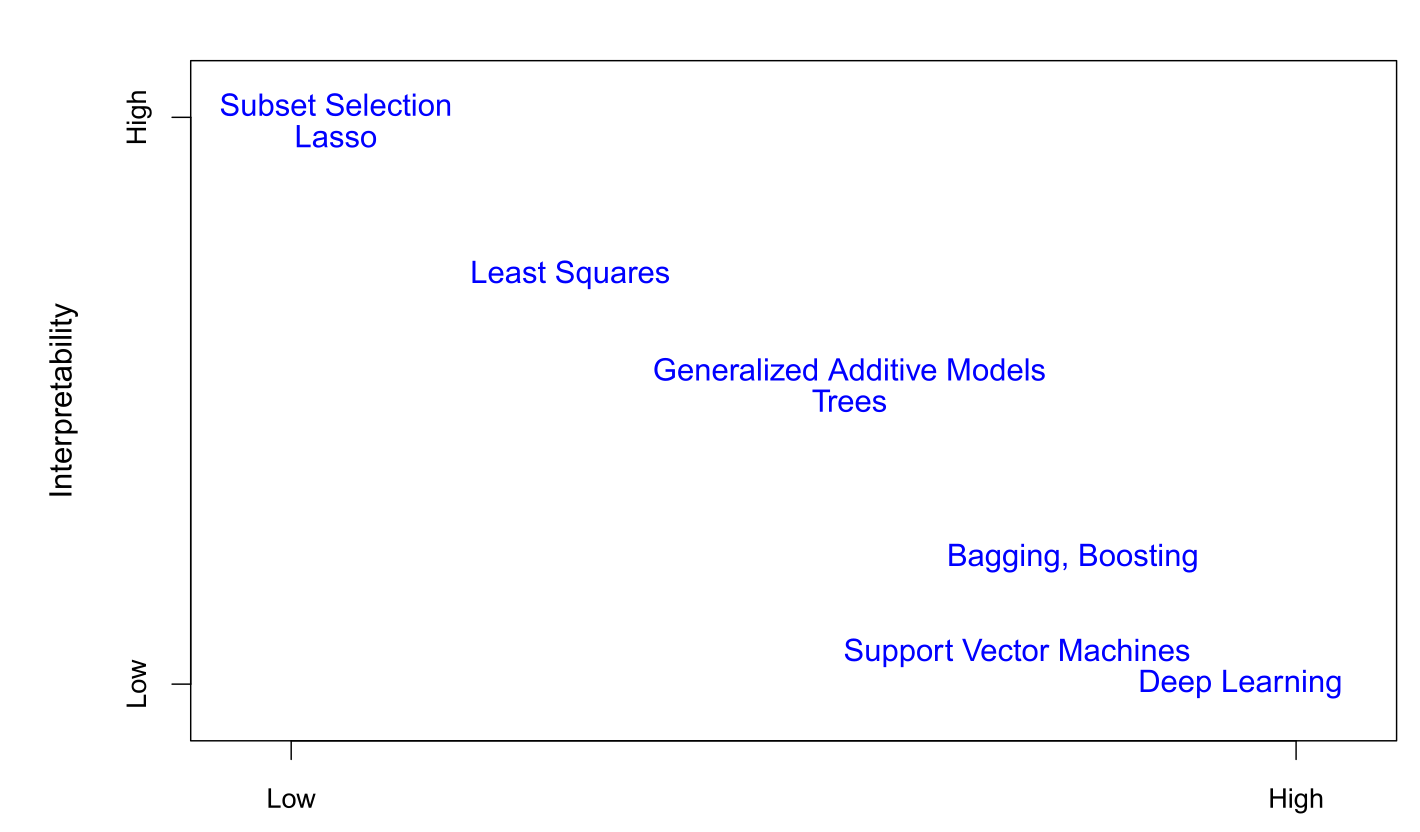
\includegraphics[scale=0.25]{./images/interpretability_vs_flexibility.png}
	\caption{Trade-off between interpretabilty and model flexibility \cite{james2013introduction}} 
\end{figure}

Neuro-symbolic models can be broadly defined as models which focus on merging both \textit{neural} and \textit{symbolic} AI approaches to add value to the system. The term \textit{nerual} refers to the use of artificial neural networks and the term \textit{symbolic} typically refers to approaches based on explicit symbol manipulation. (CITATION taxonomy.pdf) The fundamental desire of neuro-symbolic models is to leverage both neural and symbolic approaches in a way that is favorable to the strengths of each approach and unfavorable to their weaknesses. The strengths neural models would include the ability to leverage raw data that may be too dificult/complex to semantically reason about, while the weaknesses may include the challenges faced when attempting to reason neural models. Conversely, the strengths of symbolic models include their ability to be highly explainable and verifiable, but they may have weaknesses in their reliance human input/understanding of a system. Thus, the promise of a neuro-symbolic architecture is a system which would be robust from training data, symbolically explainable, and be able to leverage human expert knowledge in its design. 

In recent years many different neuro-symbolic models have been designed and deployed. Because the intersection of these two approaches may be quite broad and models can take many different forms be it is important to make distinctions between the various incarnations of neuro-symbolic architectures. Henry Kautz, in a 2005 article presents "six possible designs" patterns classifying each method in reference to their neural and symbolic interactions:(CITATION KAUTZ)

\subsection{Classification of Neuro-symbolic Architectures} \label{ss:classification}
\begin{scriptsize}
	\begin{center}
		\begin{tabular}{ | m{5cm} | m{5cm}| m{5cm} | }
			\hline
			\textbf{Neuro-symbolic Design Pattern} & \textbf{Definition} & \textbf{Example}\\
			\hline
			Symbolic Neural symbolic & A symbolic input is fed into a neural network producing a symbolc output. & GPT \\
			\hline
			Symbolic[Neural] & A neural subroutine is evoked by a symbolic strategy. & AlphaGo \\
			\hline
			Neural[Symbolic] & A symbolic subroutine is evoked by a neural strategy. & ChatGPT accessing Wolfram for computations\\
			\hline
			Neural|Symbolic & A neural network converts a non-symbolic input into symbolic data to be symbolically processed. & Neuro-Symbolic Concept Learner \\
			\hline
			Neural:Symbolic $\rightarrow$ Neural & A symbolically represented dataset is used to train an neural network to predict a symbolic output & ANN-MPC \\
			\hline
			Neural\_\{Symbolic\} & Symbolic rules are used to define the structures making up the neural network. & Logic Tensor Networks \\
			\hline
		\end{tabular}
	\end{center}
\end{scriptsize}
\subsection{Neuro-symbolic Concept Learner} \label{ss:neurosymbolic_concept_learner}
The Neuro-Symbolic Concept Learner (NS-CL), developed by Mao et al., is a representative example of the Neural|Symbolic pattern. It combines convolutional and recurrent networks to extract structured representations from images and language, which are then processed by a symbolic reasoning module. This thesis adapts NS-CL to preprocess environment observations and task instructions for reinforcement learning.

\section{Neuro-symbolic Reinforcement Learning} \label{se:neurosymbolic_rl}
Neuro-symbolic reinforcement learning (NSRL) is an emerging field that merges symbolic abstraction with RL policies. The aim is to produce agents that can learn effectively from data while providing semantic interpretability. NSRL allows for modular design, generalization across tasks, and the integration of external knowledge sources (e.g., task graphs or logic rules). In this thesis, NSRL is explored through a novel adaptation of NS-CL to guide robotic agents using natural language prompts and symbolic scene representations.

% \section{Sim-to-Real} \label{se:sim_to_real}
% \subsection{Transfer Learning} \label{ss: transfer_learning}
% \subsection{Multitask Learning} \label{ss:multitask_learning}

	\chapter{Robotic Manipulator Robotic Manipulator Platform}
Given the problem space, a real-world and cooresponding simulated environment was created as a platform to train and test reinforcement learning algorithms for the neuro-symbolic architecture described in this paper and general reinforcement learning algorithms involving robotic manipulators.
The physical hardware used for this robotic manipulator is based on an open-source hardware design[CITATION], with modifications made to reduce cost while maintaining performance.
The cooresponding simulation and control of the manipulator was developed using the ROS2 middleware suite and nd Gazebo simulation enviroment enabling a flexible and reproducable setup for training, validating, and deploying algorithms.

\section{Robotic Manipulator Hardware}  \label{se:robotic_manipulator_hardware}
The physical hardware used to test the algorithms is made up of a 6-axis robot arm communicating over serial (UART) with a PC running the algorithms in a ROS2 Jazzy workspace.
The rigid components of the arm including gears and structural pieces are made of 3D-printed Polylactic Acid (PLA).
The robotic arm uses stepper motors, belts, and pulleys to articluate the 6 joints. 
The first 5 joints (J1 to J5) use bipolar NEMA 17 stepper motors, while the last joint J6, responsible for manipulating the end effector, uses a bipolar NEMA 8 stepper motor.
The belts and pulleys are "off-the-shelf" GT2 timing belts and pulleys of varying sizes, used to the torque applied to each joint (belts and pulleys connect every motor to a joint with the exception of J6).
Ball and shunt bearings of verious sizes are also used to reduce friction in the joints.

The electronic hardware is controlled by an ATmega328p microcontoller and 6 A4988 stepper motor drivers originally setup for controlling the stepper motors of a 3D-Printer.
Custom firmware was written for the microcontroller to run the 6 stepper motor drivers simultaineously with a serial (UART) inturrupt to recieve control commands from the host PC. 
\begin{figure}
	\centering
  \begin{tikzpicture}

    \node[draw,
      minimum width=2cm,
      minimum height=1.2cm,
      ] (input) at (0,0){$ROS2$};

    \node[draw,
      minimum width=2cm,
      minimum height=1.2cm,
      right=1.5cm of input
      ] (sum) {$\mu C$};

    \node[draw,
      align=center,
      minimum width=2cm,
      minimum height=1.2cm,
      right=1cm of sum 
      ]  (controller) {$Motor$\\$Drivers$};

    \node[draw,
      minimum width=2cm,
      minimum height=1.2cm,
      right=1cm of controller 
      ]  (plant) {$Robot$};

    \node[draw,
      minimum width=2cm,
      minimum height=1.2cm,
      right=1cm of plant
      ]  (encoder) {$Encoders$};

    \node[draw=none, right=1.5cm of encoder] (output) {$y$};

    \draw[->] (input.east) -- (sum.west) node[midway, above]{\tiny{$UART$}};
    \draw[->] (sum.east) -- (controller.west) node[midway, above]{$u$};
    \draw[->] (controller.east) -- (plant.west);
    \draw[->] (plant.east) -- (encoder.west);
    \draw[->] (encoder.east) -- (output.west);
    \draw[->] (output.center) ++(-1,0) |- ++(0,-1.25) -| (sum.south) node[midway, below]{};

  \end{tikzpicture}\\
	\caption{Robot servo feedback system.} 
\end{figure}


\subsection{Inverse Kinematics} \label{ss:inverse_kinematics}

\subsection{Motor Control} \label{ss:motor_control}
Bipolar stepper motors are used to move the joints of the robot, choosen for their low cost and wide availability. Stepper motors have 

A hobbiest 3D-printer stepper motor controller with custom firmware was used to reduce cost.
\begin{figure}[htb]
  \centering
  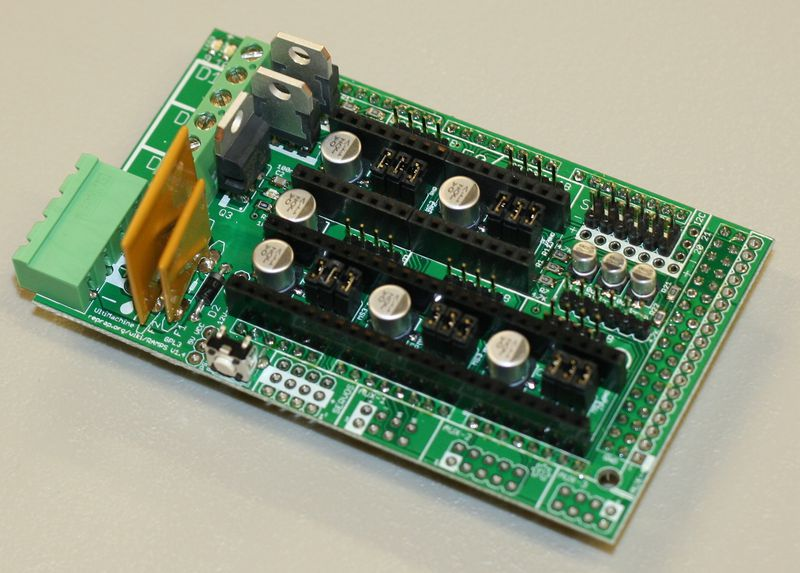
\includegraphics[scale=0.2]{RAMPS}
  \caption{RAMPS board}
  \label{fig:ramps}
\end{figure}

\subsection{Communication} \label{ss:communication}
Communication is done over a USB-UART connection, sending ROS2 position commands to a ATmega328p microcontroller used to process the position requests and update the joint positions.


\section{Robotic Manipulator Software} \label{se:virtual_overview}
The environment consists of the same six axis robot arm described in the previous section set up in the Gazebo Robotic Simulator (using a ROS Universal Robot Description File and Gazebo Simulation Description File).
Within the arm's working envelop various basic 3-D shapes (i.e. spheres, cubes, cylinders, etc.) are present.

The Robot Operating System is a middleware suite used for robot software development.
ROS workspaces consist of packages that interface with ROS libraries. 
\subsection{Robot Description} \label{ss:description_package}
The \texttt{arm\_description} package is a ROS package that contains various files used to describe the physcial characteristics of the robot including its visual, collision, control, and forward kinematics.

The six-axis robotic arm model deployed in this package is a slightly modified version of an open source six-axis robot design with modfications made to some of the pulleys and end-effector design. The robot arm is made up of six joints (J1-J6) all described as revolute joints in the \texttt{arm\_description}'s Universal Robot Description File (\texttt{.urdf}). Meshes for rendering the robot imported as \texttt{.stl} files and the meshes for collision areas are described by COLLADA (\texttt{.dae}) files. These meshes are linked together in the URDF in a kinematic chain to form the robotic arm manipulator.
Control of the robot is accomplished through the ROS Jazzy control package.
\subsection{Controllers}

\subsection{Hardware Interface}

\section{Reinforcement Learning Environment}

	\chapter{Neuro-symbolic Reinforcement Learning Model}
\section{Achitecture Overview}

\begin{figure}[htb]
	\centering
	\begin{tikzpicture}[every node/.style={align=center}, node distance=2cm]

		% Nodes
		\node[draw, thick, rectangle, rounded corners, minimum width=2cm, minimum height=1.2cm] (cnn) {CNN};
		\node[draw, thick, rectangle, rounded corners, minimum width=3cm, minimum height=2cm, right=1.5cm of cnn] (structured) {Structured \\ Representation};
		\node[draw, thick, rectangle, rounded corners, minimum width=2cm, minimum height=1.2cm, below=2cm of cnn] (rnn) {RNN};
		\node[draw, thick, rectangle, rounded corners, minimum width=3cm, minimum height=2cm, right=1.5cm of rnn] (symbolic) {Symbolic \\ Reasoning};
		\node[draw, thick, rectangle, rounded corners, minimum width=2cm, minimum height=1.2cm, right=3cm of structured] (actor) {Actor, $\mu$};
		\node[draw, thick, rectangle, rounded corners, minimum width=3cm, minimum height=1.2cm, above=2cm of actor] (environment) {Environment};
		\node[draw, thick, rectangle, rounded corners, minimum width=2cm, minimum height=1.2cm, below=2cm of actor] (critic) {Critic, $Q$};

		% Connecting Arrows
		\draw[->, thick] (cnn.east) -- (structured.west);
		\draw[->, thick] (structured.south) -- (symbolic.north);
		\draw[->, thick] (symbolic.east) -- (critic.west) node[midway, below] (state) {$s_t$, $s_{t+1}$};
		\draw[->, thick] (state.north) |- (actor.west);
		\draw[->, thick] (actor.north) -- (environment.south) node[midway, left] {$a_t$};
		\draw[->, thick] (actor.south) -- (critic.north) node[midway, left] {$a_t$, $a_{t+1}$};
		\draw[-, thick] (environment.west) -- ++(-4, 0) node[above] (invis) {} -- ++(-4, 0) node[above] (invis2) {};
		\draw[->, thick] (invis2.south) -- node[right] {Image} (cnn.north);
		\draw[->, thick] (invis.south) -- node[right] {Position} (structured.north);

		\draw[->, thick] (rnn.east) -- (symbolic.west);

		% Input and Output Arrows
		\node[left=0.8cm of rnn] (prompt) {Prompt};
		\node[right=0.8cm of critic] (Q) {$Q_{new}$};
		\draw[->, thick] (prompt.east) -- (rnn.west);
		\draw[->, thick] (critic.east) -- (Q.west);

		% Outer Box
		\draw[dashed, rounded corners] (-3.75, 4.25) rectangle (6, -4.75) node[below left] {NS-CL};
		\draw[dashed, rounded corners] (6.25, 4.25) rectangle (12.75, -4.75) node[below left] {DDPG};

	\end{tikzpicture}
  \caption{NS-CL with proposed RL adaptation.}
  \label{fig:architecture}
\end{figure}


\section{Computer Vision}
\begin{figure}[htb]
  \centering
  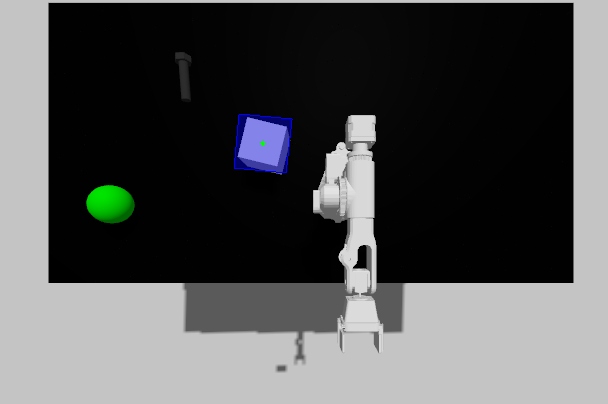
\includegraphics[scale=0.4]{cv}
  \caption{YOLOv8--OBB in Gazebo Simulation}
  \label{fig:cv}
\end{figure}

\subsection{YOLOv8--OBB}
\section{Natural Language Processing}
\section{State Representation}

\begin{figure}
	\begin{tiny}
		\begin{center}
			\begin{tabular}{ | m{2cm} | m{2cm}| m{2cm} | m{2cm} | m{3.25cm} |  }
				\hline
				\textbf{Shape} & \textbf{Color $(r, g, b)$} & \textbf{Position $(x,y)$} & \textbf{Rotation $\theta$} & \textbf{Velocity $(v_x, v_y, v_z, \omega)$} \\
				\hline
				J1 & (0, 0, 0) & (0, 0, 0) & 0\textdegree & (0, 0, 0, 0) \\ 
				\hline
				J2 & (0, 0, 0) & (0, 0.1, 0) & 0\textdegree & (0, 0, 0, 0) \\ 
				\hline
				J3 & (0, 0, 0) & (0, 0.2, 0) & 0\textdegree & (0, 0, 0, 0) \\ 
				\hline
				J4 & (0, 0, 0) & (0, 0.4, 0) & 0\textdegree & (0, 0, 0, 0) \\ 
				\hline
				J5 & (0, 0, 0) & (0, 0.4, 0) & 0\textdegree & (0, 0, 0, 0) \\ 
				\hline
				J6 & (0, 0, 0) & (0, 0.4, 0) & 0\textdegree & (0, 0, 0, 0) \\ 
				\hline
				cube & (255, 0, 255) & (0.75, 0.75, 0) & 0\textdegree & (0, 0, 0, 0) \\ 
				\hline
				cylinder & (255, 255, 0) & (-0.25, 1, 0) & 0\textdegree & (0, 0, 0, 0) \\ 
				\hline
				rectangle & (0, 0, 255) & (0.5, 0.5, 0) & 90\textdegree & (0, 0, 0, 0) \\ 
				\hline
				sphere & (0, 255, 0) & (0.6, -0.1, 0) & 0\textdegree & (0, 0, 0, 0) \\ 
				\hline
			\end{tabular}
		\end{center}
	\end{tiny}
	\caption{Example of state observation before symbolic modification.}
	\label{fig:default_state}
\end{figure}



\subsection{Symbolic Augmentations}
\begin{figure}
	\begin{tiny}
		\begin{center}
			\begin{tabular}{ | m{1cm} | m{1.75cm}| m{2cm} | m{1.5cm} | m{3cm} | m{1cm} | }
				\hline
				\textbf{Label} & \textbf{Color $(r, g, b)$} & \textbf{Position $(x,y)$} & \textbf{Rotation $\theta$} & \textbf{Velocity $(v_x, v_y, v_z, \omega)$} & \textbf{Symbol} \\
				\hline
				J1 & (0, 0, 0) & (0, 0, 0) & 0\textdegree & (0, 0, 0, 0) & null \\ 
				\hline
				J2 & (0, 0, 0) & (0, 0.1, 0) & 0\textdegree & (0, 0, 0, 0) & null\\ 
				\hline
				J3 & (0, 0, 0) & (0, 0.2, 0) & 0\textdegree & (0, 0, 0, 0) & null\\ 
				\hline
				J4 & (0, 0, 0) & (0, 0.4, 0) & 0\textdegree & (0, 0, 0, 0) & null\\ 
				\hline
				J5 & (0, 0, 0) & (0, 0.4, 0) & 0\textdegree & (0, 0, 0, 0) & null \\ 
				\hline
				J6 & (0, 0, 0) & (0, 0.4, 0) & 0\textdegree & (0, 0, 0, 0)& null \\ 
				\hline
				cube & (255, 0, 255) & (0.75, 0.75, 0) & 0\textdegree & (0, 0, 0, 0) & null\\ 
				\hline
				cylinder & (255, 255, 0) & (-0.25, 1, 0) & 0\textdegree & (0, 0, 0, 0) & avoid\\ 
				\hline
				rectangle & (0, 0, 255) & (0.5, 0.5, 0) & 90\textdegree & (0, 0, 0, 0) & move\\ 
				\hline
				sphere & (0, 255, 0) & (0.6, -0.1, 0) & 0\textdegree & (0, 0, 0, 0) & null\\ 
				\hline
				goal & (0, 0, 0) & (-1, 1, 0) & 0\textdegree & (0, 0, 0, 0) & goal\\ 
				\hline
			\end{tabular}
		\end{center}
	\end{tiny}
	\caption{Example of symbolically modified state.}
	\label{fig:symbolic_state}
\end{figure}





\section{Reinforcement Learning}
\section{Simulation Environment} \label{se:gazebo_harmonic_robotics_simulator}
    Gazebo is a robotic physics simulator developed by Open Robotics which integrates the ODE physics engine, ORGE rendering engine, and support code for sensor and actuator control integration. This environment leverages Gazebo Harmonic (the latest release of Gazebo at the time of writing) to visually render and simulate the physics of the robotic manipulator and the objects in its environment. 
\subsection{Pick and Place Simulation}
\subsection{Dataset}
The cooresponding dataset used to train the model that can be seen as an extension of the CLEVR dataset [CITATION]-- which instead prompts the agent to act on the objects in the environment.



	\chapter{Results} \label{ch:simulations}

		\chapter{Discussion} \label{ch:discussion}

	\chapter{Conclusions} \label{ch:conclusions}



	%now go ahead and start writing your thesis


	% This is the standard bibtex file. Do not include the .bib extension in <bib_file_name>.
	% Uncomment the following lines to include your bibliography: 
	%\bibliography{<bib_file_name>}
	%\bibliographystyle{plainnat}   
\end{document}


%****************************************************************************
% Below are some general suggestions for writing your dissertation:
%
% 1. Label everything with a meaningful prefix so that you
%    can refer back to sections, tables, figures, equations, etc.
%    Usage \label{<prefix>:<label_name>} where some suggested
%    prefixes are:
%			ch: Chapter
%     		se: Section
%     		ss: Subsection
%     		sss: Sub-subsection
%			app: Appendix
%     		ase: Appendix section
%     		tab: Tables
%     		fig: Figures
%     		sfig: Sub-figures
%     		eq: Equations
%
% 2. The VTthesis class provides for natbib citations. You should upload
%	 one or more *.bib bibtex files. Suppose you have two bib files: some_refs.bib and 
%    other_refs.bib.  Then your bibliography line to include them
%    will be:
%      \bibliography{some_refs, other_refs}
%    where multiple files are separated by commas. In the body of 
%    your work, you can cite your references using natbib citations.
%    Examples:
%      Citation                     Output
%      -------------------------------------------------------
%      \cite{doe_title_2016}        [18]
%      \citet{doe_title_2016}       Doe et al. [18]
%      \citet*{doe_title_2016}      Doe, Jones, and Smith [18]
%
%    For a complete list of options, see
%      https://www.ctan.org/pkg/natbib?lang=en
%
% 3. Here is a sample table. Notice that the caption is centered at the top. Also
%    notice that we use booktabs formatting. You should not use vertical lines
%    in your tables.
% 
%				\begin{table}[htb]
%					\centering
%					\caption{Approximate computation times in hh:mm:ss for full order 						versus reduced order models.}
%					\begin{tabular}{ccc}
%						\toprule
%						& \multicolumn{2}{c}{Computation Time}\\
%						\cmidrule(r){2-3}
%						$\overline{U}_{in}$ m/s & Full Model & ROM \\
%						\midrule
%						0.90 & 2:00:00 & 2:08:00\\
%						0.88 & 2:00:00 & 0:00:03\\
%						0.92 & 2:00:00 & 0:00:03\\
%						\midrule
%						Total & 6:00:00 & 2:08:06\\
%						\bottomrule
%					\end{tabular}
%					\label{tab:time_rom}
%				\end{table}
% 
% 4. Below are some sample figures. Notice the caption is centered below the
%    figure.
%    a. Single centered figure:
%					\begin{figure}[htb]
%						\centering
%						\includegraphics[scale=0.5]{my_figure.eps}
%						\caption{Average outlet velocity magnitude given an average  
%				        input velocity magnitude of 0.88 m/s.} 
%						\label{fig:output_rom}
%					\end{figure}
%    b. Two by two grid of figures with subcaptions
%					\begin{figure}[htb]
%						\centering
%						\begin{subfigure}[h]{0.45\textwidth}
%							\centering
%							\includegraphics[scale=0.4]{figure_1_1.eps}
%							\caption{Subcaption number one}
%							\label{sfig:first_subfig}
%						\end{subfigure}
%						\begin{subfigure}[h]{0.45\textwidth}
%							\centering
%							\includegraphics[scale=0.4]{figure_1_2.png}
%							\caption{Subcaption number two}
%							\label{sfig:second_subfig}
%						\end{subfigure}
%
%						\begin{subfigure}[h]{0.45\textwidth}
%							\centering
%							\includegraphics[scale=0.4]{figure_2_1.pdf}
%							\caption{Subcaption number three}
%							\label{sfig:third_subfig}
%						\end{subfigure}
%						\begin{subfigure}[h]{0.45\textwidth}
%							\centering
%							\includegraphics[scale=0.4]{figure_2_2.eps}
%							\caption{Subcaption number four}
%							\label{sfig:fourth_subfig}
%						\end{subfigure}
%						\caption{Here is my main caption describing the relationship between the 4 subimages}
%						\label{fig:main_figure}
%					\end{figure}
%
%----------------------------------------------------------------------------
%
% The following is a list of definitions and packages provided by VTthesis:
%
% A. The following packages are provided by the VTthesis class:
%      amsmath, amsthm, amssymb, enumerate, natbib, hyperref, graphicx, 
%      tikz (with shapes and arrows libraries), caption, subcaption,
%      listings, verbatim
%
% B. The following theorem environments are defined by VTthesis:
%      theorem, proposition, lemma, corollary, conjecture
% 
% C. The following definition environments are defined by VTthesis:
%      definition, example, remark, algorithm
%
%----------------------------------------------------------------------------
%
%  I hope this template file and the VTthesis class will keep you from having 
%  to worry about the formatting and allow you to focus on the actual writing.
%  Good luck, and happy writing.
%    Alan Lattimer, VT, 2016
%
%****************************************************************************
